We start by considering, in this regime, $r_0 > 0$. We know the measure \eqref{Equation: Measure Normal Matrix} to be the law for the distribution of the particles in this problem. When we say that $r_0 > 0$, we are saying that the region of space $[r_0, r_1]$ where this measure is non-zero for $N \rightarrow \infty$ has the annulus shape. If we think of the equivalent Coulomb gas, this means the particles will concentrate in this shape when we perform an asymptotic on $N$.  This is the support for the limit measure.

\begin{center}
	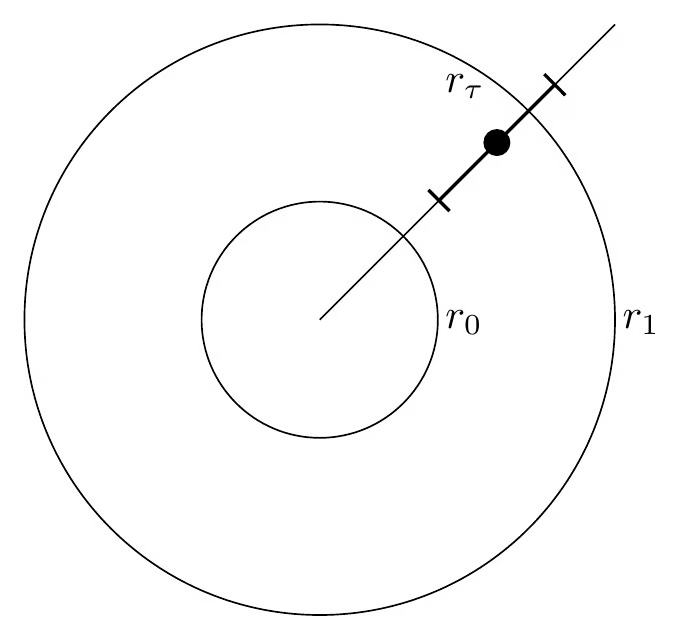
\includegraphics[width=.4\linewidth]{Assets/Annulus.png}
\end{center}

\subsubsection{Asymptotic for the orthogonal polynomial}

We begin as is usual when applying asymptotic techniques in integrals; separating a central part where the integral value is concentrated and another part where we can control the order of contribution. This is of course possible because the integrand is proportional to some exponential, with negative exponent, with a unique critical point, around which, the value of the expression concentrates. Define $\delta_N = \log(N)/\sqrt{N}$ - this will be our the cut-size for the interest region and will be justified during the calculations -, then
\begin{align}
	h_j =  \int_{|r - r_j| > \delta_N} 2r \ee^{-N V_{\tau(j)}(r)} \dd r + \int_{|r - r_j| < \delta_N} 2r \ee^{-N V_{\tau(j)}(r)} \dd r = (1) + (2).
\end{align}
As mentioned, the first integral must be somehow controlled and the second estimated as the main value for the result. 

\begin{teorema}
	We have the following asymptotic for $h_j$,
	\begin{equation}
		h_j = \frac{\ee^{-N V_{\tau(j)}(r_{\tau(j)})}}{\sqrt{N}} \left( \frac{8\pi r_{\tau(j)}^2}{V^{(2)}_{\tau_j}(r_{\tau(j)})} \right)^{\frac{1}{2}} \left[ 1 + \frac{1}{N} \mathfrak{B}_1(r_{\tau(j)}) + \Boh(N^{-2}) \right].
		\label{Equation: Asymptotic hj annulus}
	\end{equation}
	where
	\begin{equation}
	\mathfrak{B}_1(r_{\tau(j)})  = \frac{V^{(4)}_{\tau_j}(r_{\tau(j)})}{V^{(2)}_{\tau_j}(r_{\tau(j)})^2} \frac{1}{4} - \frac{V^{(3)}_{\tau_j}(r_{\tau(j)})^2}{V^{(2)}_{\tau_j}(r_{\tau(j)})^{\frac{5}{2}}} \frac{5}{12} + \frac{1}{V^{(2)}_{\tau_j}(r_{\tau(j)})} \frac{2}{3 r_{\tau(j)}}
	\end{equation}
\end{teorema}
\begin{proof}
Let's first show that we can control the first part of the integral, for that, rewrite
\begin{align}
	(1) & = \ee^{-N V_{\tau(j)}(r_{\tau(j)})} \int_{|r - r_j| > \delta_N} 2r \ee^{-N \left( V_{\tau(j)}(r) - V_{\tau(j)}(r_{\tau(j)}) \right)} \dd r, \\
	& = \ee^{-N V_{\tau(j)}(r_{\tau(j)})} \int_{|r - r_j| > \delta_N} 2r \ee^{-N \left( V_{\tau(j)}(r) - V_{\tau(j)}(r_{\tau(j)}) \right)}  \ee^{-(M-M) \left( V_{\tau(j)}(r) - V_{\tau(j)}(r_{\tau(j)}) \right)} \dd r, \\
	& = \ee^{-N V_{\tau(j)}(r_{\tau(j)})} \int_{|r - r_j| > \delta_N} 2r \ee^{-M \left( V_{\tau(j)}(r) - V_{\tau(j)}(r_{\tau(j)}) \right)}  \ee^{-(N-M) \left( V_{\tau(j)}(r) - V_{\tau(j)}(r_{\tau(j)}) \right)} \dd r.
\end{align}
Now, we need some way to estimate the difference $(V_{\tau(j)}(r) - V_{\tau(j)}(r_{\tau(j)})$. If we are able to say that this difference is at least $\Boh(N^{-1})$, we could control the growth of the integral choosing $M$ to be large enough such that
\begin{equation}
	\int_{|r - r_j| > \delta_N} \left( \ee^{-q(r)} r^{2 \tau(j)} \right)^M r \dd r
\end{equation}
converges. Using the definition of the function $V$ and the mean value theorem, we start by evaluating the difference $	V_{\tau(j+1)}(r_{\tau(j+1)}) - V_{\tau(j)}(r_{\tau(j)})$, is the following manner
\begin{align}
	V_{\tau(j+1)}(r_{\tau(j+1)}) - V_{\tau(j)}(r_{\tau(j)}) &= q(r_{\tau(j+1)}) - q(r_{\tau(j)}) - 2 \left( \tau(j+1) \log(r_{\tau(j+1)}) - \tau(j) \log(r_{\tau(j)}) \right), \\
	& = q'(c) (r_{\tau(j+1)} - r_{\tau(j)}) - \frac{2}{N} \left(\log(r_{\tau(j+1)})+j\log\left(\frac{r_{\tau(j+1)}}{r_{\tau(j)}} \right) \right), \\
	& = q'(c) r'(c) (\tau(j+1) - \tau(j)) - \frac{2}{N} \left(\log(r_{\tau(j+1)})+j \Boh(N^{-1}) \right), \\
	& = q'(c) r'(c) \Boh(N{-1}) - \Boh(N^{-1}), \\
	& = \Boh(N^{-1}).
\end{align}
The last equality holds as both functions are continuous and $c$ is some value that is limit by some compact disk on the plane. Then, we can add zero and use the estimation
\begin{equation}
	V_{\tau(j+1)}(r_{\tau(j+1)})  - V_{\tau(j+1)}(r) + V_{\tau(j+1)}(r) - V_{\tau(j)}(r_{\tau(j)}) = \Boh(N^{-1}).
\end{equation}
to derive the result we are after. It is enough to estimate $V_{\tau(j+1)}(r) - V_{\tau(j)}(r_{\tau(j)})$. For that, because $r q'(r)$ is increasing, for all $r > r_{\tau(j)} + \delta_N$ we can say that
\begin{equation}
	V_{\tau(j+1)}(r) \geq V_{\tau(j+1)}(r_{\tau(j)} + \delta_N) =  V_{\tau(j+1)}(r_{\tau(j+1)}) + \frac{1}{2} V''_{\tau(j+1)}(r_{\tau(j+1)}) (r_{\tau(j)} + \delta_N - r_{\tau(j+1)})^2 + \Boh(\delta_N^3),
\end{equation} 
and therefore can write that
\begin{align}
	V_{\tau(j+1)}(r) - V_{\tau(j)}(r_{\tau(j)}) & =  \frac{1}{2} V''_{\tau(j+1)}(r_{\tau(j+1)}) (r_{\tau(j)} + \delta_N - r_{\tau(j+1)})^2 + \Boh(\delta_N^3) \\
	& = \delta^2 c + \Boh(N^{-1}) + \Boh(\delta_N^3) \\
	& \geq  \delta^2 c
\end{align}
Finally, using this one can write
\begin{equation}
	V_{\tau(j+1)}(r) - V_{\tau(j+1)}(r_{\tau(j+1)}) \geq c \delta_N^2.
\end{equation}


%We first notice that $V_{\tau(j)}(r)$ has a critical (minimal) point at $r_{\tau(j)}$, the unique number which satisfies $r_\tau q(r_\tau) = 2 \tau$. As it will be relevant very soon in terms of laplace technique, it is worth mentioning the derivatives for $V_\tau(r)$,
%\begin{align}
%& V'_\tau(r) = q'(r) - \frac{2\tau}{r}, \\
%& V''_\tau(r) = 4 \Delta Q(r) - \frac{1}{r} V'_\tau(r).
%\end{align}
%where
%\begin{align}
%	& V'_\tau(r(\tau)) = q'(r(\tau)) - \frac{2\tau}{r(\tau)} = 0 \\
%	& V''_\tau(r(\tau)) = 4 \Delta Q(r(\tau)) - \frac{1}{r(\tau)} V'_\tau(r(\tau)) > 0.
%\end{align}
%Moreover, we have that
%\begin{equation}
%	\frac{\dd r}{\dd \tau} = \frac{2}{(r q'(r))'} |_{r = r(\tau)} = \frac{1}{2 r(\tau) \Delta Q (r(\tau))} > 0.
%\end{equation}
%Another inequality needed is that we also have $r_{\tau(j+1/2)} - r_{\tau(j)} = \Boh(N^{-1})$, for some $r_{\tau(j)}< c <r_{\tau(j+1/2)}$, you can get this inequality doing the following
%\begin{align}
%	r_{\tau(j+1/2)} - r_{\tau(j)} & = r'(c) \left( \tau\left(j+\frac{1}{2}\right) - \tau(j)\right)	\\
%	& = r'(c) \frac{j}{2N} \\
%	& = \frac{j}{2N} \frac{1}{2 r(c) \Delta Q (r(c))} \\
%	&  = \frac{j}{2N} \frac{2}{q'(r(c)) + r(c) q''(r(c))} \\
%	& = \frac{j}{2N} \frac{2}{\frac{\dd (r q'(r))}{\dd r}|_{r = r(c)}} > 0 \\
%	& = \Boh(N^{-1}).
%\end{align}
%Using this properties we can also deduce that $V_{\tau(j+\frac{1}{2})} - V_{\tau(j)} = \Boh(N^{-1})$, that we can show as follows
%\begin{align}
%	V_{\tau(j+\frac{1}{2})} - V_{\tau(j)} &= q(r_{\tau(j+\frac{1}{2})}) - q(r_{\tau(j)}) - 2 \left( \tau(j+\frac{1}{2}) \log(r_{\tau(j+\frac{1}{2})}) - \tau(j) \log(r_{\tau(j)}) \right) \\
%	& = q'(c) (r_{\tau(j+\frac{1}{2})} - r_{\tau(j)}) - 2 \left( \left(r_{\tau(j+\frac{1}{2})} - r_{\tau(j)} \right) \log(r_{\tau(j+\frac{1}{2})}) + \tau(j) \log\left( \frac{r_{\tau(j+\frac{1}{2})}}{r_{\tau(j)}}  \right) \right) \\
%	& = \Boh(N^{-1}).
%\end{align}
%And finally, because $r q'(r)$ is increasing, for all $r > r_{\tau(j)} + \delta_N$ we have
%\begin{equation}
% V_{\tau(j+\frac{1}{2})}(r) \geq V_{\tau(j+\frac{1}{2})}(r_{\tau(j)} + \delta_N) =  V_{\tau(j+\frac{1}{2})}(r_{\tau(j+\frac{1}{2})}) + \frac{1}{2} V''_{\tau(j+\frac{1}{2})}(r_{\tau(j+\frac{1}{2})}) (r_{\tau(j)} + \delta_N - r_{\tau(j+\frac{1}{2})})^2 + \Boh(\delta_N^3) 
%\end{equation} 
%and therefore can write that
%\begin{align}
%	V_{\tau(j+\frac{1}{2})}(r) - V_{\tau(j)}(r_{\tau(j)}) & =  \frac{1}{2} V''_{\tau(j+\frac{1}{2})}(r_{\tau(j+\frac{1}{2})}) (r_{\tau(j)} + \delta_N - r_{\tau(j+\frac{1}{2})})^2 + \Boh(\delta_N^3) \\
%	& = \delta^2 c + \Boh(N^{-1}) + \Boh(\delta_N^3) \\
%	& \geq  \delta^2 c
%\end{align}
%or some positive real constant $c$.
Getting this inequality back to the integral expression we can write that 
\begin{align}
	(1) & =  \ee^{-N V_{\tau(j)}(r_{\tau(j)})} \int_{|r - r_j| > \delta_N} 2r \ee^{-M \left( V_{\tau(j)}(r) - V_{\tau(j)}(r_{\tau(j)}) \right)}  \ee^{-(N-M) \left( V_{\tau(j)}(r) - V_{\tau(j)}(r_{\tau(j)}) \right)} \dd r \\
	& = \ee^{-N V_{\tau(j)}(r_{\tau(j)})}  \ee^{- c \delta_N^2 (N - M)} \int_{|r - r_j| > \delta_N} 2r \ee^{-M \left( V_{\tau(j)}(r) - V_{\tau(j)}(r_{\tau(j)}) \right)} \dd r
\end{align}
where you can check that
\begin{align}
	\int_{|r - r_j| > \delta_N} 2r \ee^{-M \left( V_{\tau(j)}(r) - V_{\tau(j)}(r_{\tau(j)}) \right)} \dd r & = \int_{|r - r_j| > \delta_N} 2r \ee^{-M \left( (q(r) - 2 \tau(j) \log(r)) - (q(r_{\tau(j)}) - 2 \tau(j) \log(r_{\tau(j)})) \right)} \dd r  \\
	& = 2 \left( \ee^{-q(r_{\tau(j)})} r_{\tau(j)}^{-2 \tau(j)} \right)^M \int_{|r - r_j| > \delta_N} \left( \ee^{-q(r)} r^{2 \tau(j)} \right)^M r \dd r.
\end{align}
We chose $M$ to be a big enough number such that the integral above converges. If that is true, 
\begin{equation}
	(1) = \int_{|r - r_j| > \delta_N} 2r \ee^{-N V_{\tau(j)}(r)} \dd r = \ee^{-N V_{\tau(j)}(r_{\tau(j)})} \epsilon_N
\end{equation}
with $\epsilon_N = \Boh(\ee^{-c(\log(N))^2})$.  

Now we must deal with the second part of the integral. We begin be setting $x = r - r_\tau$, then
\begin{align}
	(2) & = \int_{-\delta_N}^{\delta_N} 2 (x + r_{\tau_j}) \ee^{-N V_{\tau(j)}(x + r_{\tau(j)})} \dd x \\
	& = \ee^{-N V_{\tau(j)}(r_{\tau(j)})}  \int_{-\delta_N}^{\delta_N} 2 (x + r_{\tau_j}) \ee^{-N \left[ V_{\tau(j)}(x + r_{\tau(j)}) - V_{\tau(j)}(r_{\tau(j)})\right]} \dd x
\end{align}
By re-scaling the integral using $y = \sqrt{N} x$ we get yet
\begin{equation}
	(2) = \frac{\ee^{-N V_{\tau(j)}(r_{\tau(j)})}}{\sqrt{N}}  \int_{-\log(N)}^{\log(N)} 2 \left(\frac{y}{\sqrt{N}} + r_{\tau_j} \right) \ee^{-N \left[ V_{\tau(j)}(\frac{y}{\sqrt{N}} + r_{\tau(j)}) - V_{\tau(j)}(r_{\tau(j)})\right]} \dd y
\end{equation}
Now, the idea here is quite direct: to use the Taylor expansion for $V_{\tau(j)}\left(\frac{y}{\sqrt{N}} + r_{\tau(j)}\right )$ near the critical point $r_{\tau(j)}$. That is,  
\begin{align}
	(2) & =\frac{\ee^{-N V_{\tau(j)}(r_{\tau(j)})}}{\sqrt{N}}  \int_{-\log(N)}^{\log(N)} 2 \left(\frac{y}{\sqrt{N}} + r_{\tau_j} \right) \ee^{-N \left(\frac{y^2}{2N} V^{(2)}_{\tau_j}(r_{\tau(j)}) + \frac{y^3}{3! N^{\frac{3}{2}}} V^{(3)}_{\tau(j)}(r_{\tau(j)}) + \frac{y^4}{4! N^2} V^{(4)}_{\tau(j)}(r_{\tau(j)})+ \Boh\left(\left(\frac{y}{\sqrt{N}}\right)^5\right) \right)} \dd y \\
	& = 2 r_{\tau(j)} \frac{\ee^{-N V_{\tau(j)}(r_{\tau(j)})}}{\sqrt{N}}  \int_{-\log(N)}^{\log(N)} \left(\frac{y}{r_{\tau(j)}\sqrt{N}} + 1 \right) \ee^{-\frac{y^2}{2} V^{(2)}_{\tau_j}(r_{\tau(j)}) - \frac{y^3}{3! \sqrt{N}} V^{(3)}_{\tau(j)}(r_{\tau(j)}) - \frac{y^4}{4! N} V^{(4)}_{\tau(j)}(r_{\tau(j)}) + \Boh\left(\frac{y^5}{N^\frac{3}{2}}\right)} \dd y \\
	& = 2 r_{\tau(j)} \frac{\ee^{-N V_{\tau(j)}(r_{\tau(j)})}}{\sqrt{N}}  \int_{-\log(N)}^{\log(N)} \left(\frac{y}{r_{\tau(j)}\sqrt{N}} + 1 \right) \ee^{-\frac{y^2}{2} V^{(2)}_{\tau_j}(r_{\tau(j)})} \left(\ee^{- \frac{y^3}{3! \sqrt{N}} V^{(3)}_{\tau(j)}(r_{\tau(j)}) - \frac{y^4}{4! N} V^{(4)}_{\tau(j)}(r_{\tau(j)}) + \Boh\left(\frac{y^5}{N^\frac{3}{2}}\right)}\right) \dd y
\end{align}
Now we take the Taylor Series for 
\begin{align}
	& \ee^{- \frac{y^3}{3! \sqrt{N}} V^{(3)}_{\tau(j)}(r_{\tau(j)}) - \frac{y^4}{4! N} V^{(4)}_{\tau(j)}(r_{\tau(j)}) + \Boh\left(\frac{y^5}{N^\frac{3}{2}}\right)} = 1 - \left[ \frac{y^3}{3! \sqrt{N}} V^{(3)}_{\tau(j)}(r_{\tau(j)}) + \frac{y^4}{4! N} V^{(4)}_{\tau(j)}(r_{\tau(j)}) + \Boh\left(\frac{y^5}{N^\frac{3}{2}}\right) \right]  \\ 
	& - \frac{1}{2} \left[ \frac{y^6}{N} \left(\frac{V^{(3)}_{\tau(j)}(r_{\tau(j)})}{6} \right)^2 + \frac{y^8}{N^2} \left(\frac{V^{(4)}_{\tau(j)}(r_{\tau(j)})}{24} \right)^2 + \frac{y^7}{N^3} \left(\frac{V^{(4)}_{\tau(j)}(r_{\tau(j)})}{6} \frac{V^{(3)}_{\tau(j)}(r_{\tau(j)})}{24} \right) + \Boh\left(\frac{y^8}{N^2}\right)  \right] + \Boh\left(\frac{y^a}{N^b}\right)
\end{align}
to get the asymptotic expansion (since odd terms vanish) we reorganize
\begin{align}
	(2) & = 2 r_{\tau(j)} \frac{\ee^{-N V_{\tau(j)}(r_{\tau(j)})}}{\sqrt{N}}  \int_{-\log(N)}^{\log(N)} \ee^{-\frac{y^2}{2} V^{(2)}_{\tau_j}(r_{\tau(j)})}  \left[ 1 - \frac{y^4}{3! r_{\tau(j)} N} V^{(3)}_{\tau(j)}(r_{\tau(j)}) - \frac{y^4}{4! N} V^{(4)}_{\tau(j)}(r_{\tau(j)}) - \frac{y^6}{2 \cdot (3!)^2 N} V^{(3)}_{\tau(j)}(r_{\tau(j)})^2 \right] \dd y \\
\end{align}
then
\begin{align}
	(2) = 2 r_{\tau(j)} \frac{\ee^{-N V_{\tau(j)}(r_{\tau(j)})}}{\sqrt{N}} 
	& \scalebox{2}{[}
	\left(- \frac{V^{(4)}_{\tau(j)}(r_{\tau(j)})}{24 N} - \frac{V^{(3)}_{\tau(j)}(r_{\tau(j)})}{6 r_{\tau(j)} N} \right)
	\int_{-\log(N)}^{\log(N)} \ee^{-\frac{y^2}{2} V^{(2)}_{\tau_j}(r_{\tau(j)})} y^4 \\
	& - \frac{V^{(3)}_{\tau(j)}(r_{\tau(j)})^2}{72 N}
	\int_{-\log(N)}^{\log(N)} \ee^{-\frac{y^2}{2} V^{(2)}_{\tau_j}(r_{\tau(j)})} y^6 +
	\int_{-\log(N)}^{\log(N)} \ee^{-\frac{y^2}{2} V^{(2)}_{\tau_j}(r_{\tau(j)})} \scalebox{2}{]}
\end{align}
the result can be directly evaluated using the Gaussian integrals
\begin{equation}
	\int_{\R} \ee^{-2ar^2} \dd r = \sqrt{\frac{\pi}{2}} \frac{1}{a^{1/2}} \quad \implies \quad \int_{\R} \ee^{- 2 \left( \frac{V^{(2)}_{\tau_j}(r_{\tau(j)})}{4} \right) y^2} = \sqrt{\frac{\pi}{2}} \left( \frac{4}{V^{(2)}_{\tau_j}(r_{\tau(j)})} \right)^{\frac{1}{2}}
\end{equation}
\begin{equation}
	\int_{\R} \ee^{-2ar^2} r^4 \dd r = \sqrt{\frac{\pi}{2}} \frac{3}{16} \frac{1}{a^{5/2}} \quad \implies \quad \int_{\R} \ee^{- 2 \left( \frac{V^{(2)}_{\tau_j}(r_{\tau(j)})}{4} \right) y^2} y^4 = \sqrt{\frac{\pi}{2}} \frac{3}{16} \left(\frac{4}{V^{(2)}_{\tau_j}(r_{\tau(j)})} \right)^{\frac{5}{2}}
\end{equation}
\begin{equation}
	\int_{\R} \ee^{-2ar^2} r^6 \dd r = \sqrt{\frac{\pi}{2}} \frac{15}{64} \frac{1}{a^{7/2}} \quad \implies \quad \int_{\R}\ee^{- 2 \left( \frac{V^{(2)}_{\tau_j}(r_{\tau(j)})}{4} \right) y^2} y^6 = \sqrt{\frac{\pi}{2}} \frac{15}{64} \left( \frac{4}{V^{(2)}_{\tau_j}(r_{\tau(j)})} \right)^{\frac{7}{2}}
\end{equation}
we can finally calculate
\begin{align}
	(2) = \sqrt{2\pi} r_{\tau(j)} \frac{\ee^{-N V_{\tau(j)}(r_{\tau(j)})}}{\sqrt{N}} 
	& \scalebox{2}{[}
	\left(- \frac{V^{(4)}_{\tau(j)}(r_{\tau(j)})}{24 N} - \frac{V^{(3)}_{\tau(j)}(r_{\tau(j)})}{6 r_{\tau(j)} N} \right) \left( \frac{4}{V^{(2)}_{\tau_j}(r_{\tau(j)})} \right)^{\frac{1}{2}} \\
	& - \frac{V^{(3)}_{\tau(j)}(r_{\tau(j)})^2}{72 N}
	\frac{3}{16} \left(\frac{4}{V^{(2)}_{\tau_j}(r_{\tau(j)})} \right)^{\frac{5}{2}} +
	\frac{15}{64} \left( \frac{4}{V^{(2)}_{\tau_j}(r_{\tau(j)})} \right)^{\frac{7}{2}}
	\scalebox{2}{]}
\end{align}
and rearranging the terms
\begin{equation}
	(2) =  \frac{\ee^{-N V_{\tau(j)}(r_{\tau(j)})}}{\sqrt{N}} \left( \frac{8\pi r_{\tau(j)}^2}{V^{(2)}_{\tau_j}(r_{\tau(j)})} \right)^{\frac{1}{2}} \left[ 1 + \frac{1}{N} B_1(r_{\tau(j)}) + \Boh(N^{-2}) \right]
	\label{Equation: main part annulus}
\end{equation}
where
\begin{equation}
	\mathfrak{B}_1(r_{\tau(j)})  = \frac{V^{(4)}_{\tau_j}(r_{\tau(j)})}{V^{(2)}_{\tau_j}(r_{\tau(j)})^2} \frac{1}{4} - \frac{V^{(3)}_{\tau_j}(r_{\tau(j)})^2}{V^{(2)}_{\tau_j}(r_{\tau(j)})^{\frac{5}{2}}} \frac{5}{12} + \frac{1}{V^{(2)}_{\tau_j}(r_{\tau(j)})} \frac{2}{3 r_{\tau(j)}}
\end{equation}

Notice that the error term of $(1)$ is absorbed into the error order of \ref{Equation: main part annulus}. Therefore we have the asymptotic expression for $h_j$ given by \eqref{Equation: Asymptotic hj annulus}.

\end{proof}

\subsubsection{Asymptotics on the Summation}

 So now we need to return to  \eqref{Equation: Partition Function} and calculate 
\begin{align}
	\sum_{j=0}^{N-1} \log{h_j} & = \sum_{j=0}^{N-1} -N V_{\tau(j)}(r_{\tau(j)}) + \frac{1}{2} \left(\log(8\pi r^2_{\tau(j)}) - \log N - \log V^{(2)}_{\tau_j}(r_{\tau(j)}) \right) + \frac{1}{N} \mathfrak{B}_1(r_{\tau(j)}) + \Boh(N^{-2}). 
	\label{Equation: sum log annulus}
\end{align}

\begin{teorema}
	\begin{equation}
	- 2 N^2 I_Q[\mu_Q] + N \left( 3\log(2\pi) - E_Q[\mu_Q] - 1\right) + \frac{1}{2} \log(N) + 2 \int_S \mathfrak{B}_1 \dd \mu_Q + \Boh(N^{-1})
	\end{equation}
	where we have set
\begin{equation}
	\mathfrak{B}_1(r_{\tau(j)})  = \frac{V^{(4)}_{\tau_j}(r_{\tau(j)})}{V^{(2)}_{\tau_j}(r_{\tau(j)})^2} \frac{1}{4} - \frac{V^{(3)}_{\tau_j}(r_{\tau(j)})^2}{V^{(2)}_{\tau_j}(r_{\tau(j)})^{\frac{5}{2}}} \frac{5}{12} + \frac{1}{V^{(2)}_{\tau_j}(r_{\tau(j)})} \frac{2}{3 r_{\tau(j)}},
\end{equation}
\begin{equation}
	I_Q[\mu_Q] = \left[\frac{1}{4} \int_{r_0}^{r_1} q(s) s V^{(2)}_{\tau_j}(s) \dd s- \log(r_1) + \frac{1}{2} q(r_1) \right] 
\end{equation}
and
\begin{equation}
	E_Q[\mu_Q] = \frac{1}{2} \int_{r_0}^{r_1} \log(V^{(2)}(s)) (sq'(s))' \dd s.
\end{equation}
\end{teorema}

\begin{proof}

For each term depending on $j$ we need an summation expression, we first look at the first term using the Euler-Maclaurin formula
\begin{equation}
	\sum_{j=0}^{N-1} V_{\tau(j)}(r_{\tau(j)}) = \int_0^N V_{\tau(j)}(r_{\tau(j)})  \dd t - \frac{1}{2} \left( V_{\tau(j)}(r_{\tau(j)})  - V_{\tau(0)}(r_{\tau(0)}) \right) + \frac{1}{12} \left[ \partial_t V_{\tau(j)}(r_{\tau(j)}) |_{t=N} - \partial_t V_{\tau(j)}(r_{\tau(j)}) |_{t=0} \right] + \Boh(N^{-3}).
	\label{Equation: EulerMaclaurin 1 annulus}
\end{equation}
The first term in \eqref{Equation: EulerMaclaurin 1 annulus} is solved doing a integral by parts. We remember the expression for the potential $V_{\tau(j)}(r_{\tau(j)}) = q(r_{\tau(j)}) - 2 \tau(j) \log r$, with $\tau(j) = j/N$. Therefore the differential can be written as
\begin{align}
	\dd( r_{\tau(j)} q'(r_{\tau(j)}) ) & = 2 \dd \tau(j) \\
	\dd r q'(r) + \dd r r q''(r) & = 2 \dd \tau(j) \\
	\dd r (q'(r) + r q''(r)) & = 2 \dd \tau(j).
\end{align}
This implies that the derivative for $r$ is
\begin{equation}
	\frac{\dd r}{\dd \tau} = \frac{2}{r_{\tau(j)} V^{(2)}_{\tau_j}(r_{\tau(j)})} = \frac{2}{(r q'(r))'}.
\end{equation}
Note that in the critical point $r_{\tau(j)}$, we should have $r_{\tau(j)} q'(r_{\tau(j)}) = 2 \tau$. We then are able to rewrite, setting $s = r_{\tau(j)}$,
\begin{align}
	\int_0^N V_{\tau(t)}(r_{\tau(t)})  \dd t & = \int_0^N (q(r_{\tau(t)}) - 2 \tau(t) \log(r_{\tau(t)})) \dd t \\
	& = \frac{1}{2} \int_{r_0}^{r_1} (q(s) - s q'(s) \log(s)) s V^{(2)}_{\tau_j}(s) N \dd s \\
	& = N \left[  \frac{1}{2} \int_{r_0}^{r_1} q(s) s V^{(2)}_{\tau_j}(s) \dd s -  \frac{1}{2} \int_{r_0}^{r_1} s^2 q'(s) \log(s) V^{(2)}_{\tau_j}(s) \dd s \right]
\end{align}
and finally using that $r_1 q'(r_1) = 2$ and $r_0 q'(r_0) = 0$ we can apply the integration by parts on the second term and get
\begin{align}
	\frac{1}{2} \int_{r_0}^{r_1} s^2 q'(s) \log(s) V^{(2)}_{\tau_j}(s) \dd s & = \frac{1}{2} \int_{r_0}^{r_1} s^2 q'(s) \log(s) \frac{1}{s} (s q'(s))' \dd s \\
	&= \frac{1}{2} \int_{r_0}^{r_1} s q'(s) \log(s) (s q'(s))' \dd s \\
	& = \frac{1}{4} \int_{r_0}^{r_1} ((sq'(s))^2)' \log(s) \dd s \\
	& = \frac{1}{4} (s q'(s))^2 \log(s) |_{r_0}^{r_1} + \frac{1}{4}  \int_{r_0}^{r_1} (s q'(s))^2 \frac{1}{s} \dd s \\
	& = \log(r_1) + \frac{1}{4} \int_{r_0}^{r_1} s q'(s)^2 \dd s \\
	& = \log(r_1) + \frac{1}{2} q(r_1) - \frac{1}{4} \int_{r_0}^{r_1} q(s) (s q'(s))' \dd s
\end{align}
Leaving us with
\begin{align}
	\int_0^N V_{\tau(j)}(r_{\tau(j)})  \dd t & = N \left[\frac{1}{2} \int_{r_0}^{r_1} q(s) s V^{(2)}_{\tau_j}(s) \dd s - \log(r_1) + \frac{1}{2} q(r_1) - \frac{1}{4} \int_{r_0}^{r_1} q(s) (s q'(s))' \dd s \right]  \\
	& = N \left[\frac{1}{4} \int_{r_0}^{r_1} q(s) s V^{(2)}_{\tau_j}(s) \dd s- \log(r_1) + \frac{1}{2} q(r_1) \right]  \\
	& \deff N I_Q[\mu_Q]  
	\label{Equation: Equilibrium energy annulus}
\end{align}
We also need an expression for $ V_{\tau(j)}(r_{\tau(j)})  - V_{\tau(0)}(r_{\tau(0)})$. This is direct noting that
\begin{equation}
	V_{\tau(j)}(r_{\tau(j)})  - V_{\tau(0)}(r_{\tau(0)}) = V_1(r_1) - V_0(r_0) = q(r_1) - q(r_0) - 2 \log(r_1) =: 2 U_{\mu_Q}(0)
	\label{Equation: U function annulus}
\end{equation}
And finally we can the remaining term , we use the Leibniz rule and obtain
\begin{align}
	\partial_t V_{\tau(t)}(r_{\tau(t)})|_{t=N}	& = \partial_t \left( q(r_{\tau(t)}) - 2 \tau(t) \log(r_{\tau(t)}) \right)_{t=N} \\
	& = \partial_\tau \left( q(r_{\tau(t)}) - 2 \tau(t) \log(r_{\tau(t)}) \right)_{\tau=1} \partial_t \left( \tau(t) \right)_{t =N} \\
	& = \frac{1}{N} \left( \partial_\tau (q(r_{\tau})) - 2 \left( \log(r_{\tau}) + \tau \partial_\tau\left( \log(r_{\tau}) \right)_{\tau = 1} \right) \right) \\
	& = \frac{1}{N} \left[ \partial_t(q(r_{\tau(t)}) - 2 \log(r_{\tau(t)}))_{\tau=1} - 2 \log(r_1) \right] 
\end{align}
and
\begin{equation}
	\partial_t V_{\tau(t)}(r_{\tau(t)})|_{t=0} = \frac{1}{N} \left[ \partial_t(q(r_{\tau(t)}) - 2 \log(r_{\tau(t)}))_{\tau= 0} - 2 \log(r_0) \right].
\end{equation}
And since we can calculate, from $r_1 q'(r_1) = 2$ and $r_0 q'(r_0) = 0$
\begin{equation}
	\partial_\tau q(r_{\tau}) |_{\tau = 0} = \left( \frac{2 q'(r)}{(r q'(r))'}\right)_{r_0} = 0,
\end{equation}
\begin{equation}
	\partial_\tau q(r_{\tau}) |_{\tau = 1} = \left( \frac{2 q'(r)}{(r q'(r))'}\right)_{r_1} = \frac{4}{r_1(q'(r_1) + r_1 q''(r_1))},
\end{equation}
\begin{equation}
	\partial_\tau (2 \log(r_\tau)) |_{\tau = 1} = \left( \frac{4}{r (r q'(r))'}\right)_{r_1} = \frac{4}{r_1(q'(r_1) + r_1 q''(r_1))},
\end{equation}
we can also express the difference as
\begin{equation}
	\partial_t V_{\tau(t)}(r_{\tau(t)})|_{t=N}  - \partial_t V_{\tau(t)}(r_{\tau(t)})|_{t=0} = \frac{1}{12 N} \left[ 2 (\log(r_0) - \log(r_1)) \right] = \frac{1}{6 N} \log\left(\frac{r_0}{r_1}\right) .
	\label{Equation: log annulus}
\end{equation}
And the proof for the summation $\sum_{j=0}^{N-1} V_{\tau(j)}(r_{\tau(j)})$ is complete if one gathers the terms \eqref{Equation: Equilibrium energy annulus}, \eqref{Equation: log annulus} and \eqref{Equation: U function annulus},
\begin{equation}
	- N \sum_{j=0}^{N-1} V_{\tau(j)}(r_{\tau(j)}) = - N^2 I^Q[\mu_Q] - 2 N U_{\mu_Q}(0) - \frac{1}{6} \log{\left( \frac{r_0}{r_1}\right)} + \Boh(N^{-2})
	\label{Equation: sum V annulus}
\end{equation}
We move on to the next term from where we need to determine both terms in $ \sum_{j=0}^{N-1}\left(\log(2\pi r^2_{\tau(j)}) - \log V^{(2)}_{\tau_j}(r_{\tau(j)}) \right)$. Lets start now with the second summation, to which we apply Euler-Maclaurin again
\begin{equation}
	\sum_{j=0}^{N-1}  \log V^{(2)}_{\tau_j}(r_{\tau(j)}) = \int_{0}^{N} \log V^{(2)}_{\tau_t}(r_{\tau(t)}) \dd t - \frac{1}{2} \log \left( \frac{V^{(2)}_{1}(r_1)}{V^{(2)}_{0}(r_{0})} \right) + \frac{1}{12} \left[ \partial_t \log V^{(2)}_{\tau_t}(r_{\tau(t)}) |_{t=1} - \partial_t \log V^{(2)}_{\tau_t}(r_{\tau(t)}) |_{t=0}\right]  + \Boh(N^{-3})
\end{equation}
We first tackle the integral on the right hand side, changing variables as $s = r_{\tau(t)}$ we would have
\begin{equation}
	\int_{0}^{N} \log V^{(2)}_{\tau_t}(r_{\tau(t)}) \dd t = \frac{N}{2} \int_{r_0}^{r_1} \log(V^{(2)}(s)) (sq'(s))' \dd s \\
\end{equation}
And, noticing that
\begin{equation}
	\partial_t \log V^{(2)}_{\tau_t}(r_{\tau(t)}) = \partial_V \left( \log V^{(2)}_{\tau_t}(r_{\tau(t)}) \right) \partial_r \left( V^{(2)}_{\tau_t}(r_{\tau(t)}) \right) \partial_\tau \left( r_{\tau(t)} \right) = \frac{\left(\partial_r V^{(2)}\right)(r_{\tau(t)})}{r_{\tau(t)} \left( V^{(2)}(r_{\tau(t)})\right)^2}
\end{equation}
We have for the third term on the right hand side, 
\begin{align}
	\partial_t \log V^{(2)}_{\tau_t}(r_{\tau(t)}) |_{t=1} - \partial_t \log V^{(2)}_{\tau_t}(r_{\tau(t)}) |_{t=0} = \frac{1}{2N} \left( \frac{\left(\partial_r V^{(2)}\right)(r_{1})}{r_1 \left( V^{(2)}(r_1)\right)^2} - \frac{\left(\partial_r V^{(2)}\right)(r_{0})}{r_0 \left( V^{(2)}(r_0)\right)^2}\right) = \Boh(N^{-1})
\end{align}
then,
\begin{equation}
	\sum_{j=0}^{N-1}  \log V^{(2)}_{\tau_j}(r_{\tau(j)})  = \frac{N}{2} \int_{r_0}^{r_1} \log(V^{(2)}(s)) (sq'(s))' \dd s  -   \frac{1}{2} \log \left( \frac{V^{(2)}_{1}(r_1)}{V^{(2)}_{0}(r_{0})} \right) + \Boh(N^{-1})
	\label{Equation: logV annulus}
\end{equation}
Similarly, for the first summation, we apply Euler-Maclaurin again
\begin{equation}
	\sum_{j=0}^{N-1}  \log(8 \pi r^2_{\tau(j)}) = \log(8\pi) + 2 \left( \int_{0}^{N} \log(r_{\tau(t)})  \dd t - \frac{1}{2} \log\left(\frac{r_1}{r_0}\right) + \frac{1}{12} \left[ \partial_t \log r_{\tau(t)} |_{t=1} - \partial_t \log r_{\tau(t)} |_{t=0}\right] + \Boh(N^{-3}) \right)
\end{equation}
We first tackle the integral on the right hand side, changing variables as $s = r_{\tau(t)}$ we would have
\begin{equation}
	\int_{0}^{N} \log r_{\tau(t)} \dd t = \frac{N}{2} \int_{r_0}^{r_1} \log(s) (s q'(s))' \dd s \\
\end{equation}
And, noticing that
\begin{equation}
	\partial_t \log r_{\tau(t)} =  \partial_r \left( \log(r_{\tau(t)}) \right) \partial_\tau \left( r_{\tau(t)} \right) = \frac{2}{V^{(2)}(r_{\tau(t)}) \left( r_{\tau(t)} \right)^2}
\end{equation}
We have for the third term on the right hand side, 
\begin{align}
	\partial_t \log  r_{\tau(t)} |_{t=1} - \partial_t \log  r_{\tau(t)}  |_{t=0}  = \frac{1}{2N} \left( \frac{2}{V^{(2)}(r_{1}) \left( r_{1} \right)^2} - \frac{2}{V^{(2)}(r_{0}) \left( r_{0} \right)^2} \right) = \Boh(N^{-1})
\end{align}
then
\begin{equation}
	\sum_{j=0}^{N-1}  \log(8\pi r^2_{\tau(j)}) = N \log(8\pi) + 2 \left( \frac{N}{2} \int_{r_0}^{r_1} \log(s) (s q'(s))' \dd s - \frac{1}{2} \log\left(\frac{r_1}{r_0}\right) + \Boh(N^{-1}) \right) 
	\label{Equation: log(r) annulus}
\end{equation}
With all of this, gathering the terms in \eqref{Equation: sum log annulus} with the expressions in \eqref{Equation: sum V annulus}, \eqref{Equation: logV annulus} and \eqref{Equation: log(r) annulus}, one can now finally express
\begin{equation}
	\sum_{j=0}^{N-1} \log(h_j) = - N^2 I_Q[\mu_Q] - \frac{N}{2} \log N + N \left(\frac{3\log(2\pi)}{2} - \frac{1}{2} E_Q[\mu_Q]\right) - \frac{1}{2} \log\left(\frac{r_1}{r_0} \right) + \frac{1}{4} \log\left(\frac{V^{(2)}(r_1)}{V^{(2)}(r_0)} \right) + \int_S \mathfrak{B}_1 \dd \mu_Q + \Boh(N^{-1})
\end{equation}
where
\begin{equation}
	E_Q[\mu_Q] = \frac{1}{2} \int_{r_0}^{r_1} \log(V^{(2)}(s)) (sq'(s))' \dd s 
\end{equation}
from which we can get the asymptotic expansion using that
\begin{equation}
	\log(N!) = N\log(N) - N + \frac{1}{2} \log(N) + \frac{1}{2} \log(2 \pi) + \Boh(N^{-1})
\end{equation}
that is,
\begin{align}
	\ln Z_N & = \ln{N!} - 2 \sum_{j=0}^{N-1} \log{h_j} \\
	& = N\log(N) - N + \frac{1}{2} \log(N) + \frac{1}{2} \log(2 \pi) + 2 \left( - N^2 I_Q[\mu_Q] - \frac{N}{2} \log N + N \left(\frac{3\log(2\pi)}{2} - \frac{1}{2} E_Q[\mu_Q]\right) - \frac{1}{2} \log\left(\frac{r_1}{r_0} \right) + \frac{1}{4} \log\left(\frac{V^{(2)}(r_1)}{V^{(2)}(r_0)} \right) + \int_S \mathfrak{B}_1 \dd \mu_Q \right) + \Boh(N^{-1}) \\
	& =  - 2 N^2 I_Q[\mu_Q] + N \left( 3\log(2\pi) - E_Q[\mu_Q] - 1\right) + \frac{1}{2} \log(N) + 2 \int_S \mathfrak{B}_1 \dd \mu_Q + \Boh(N^{-1})
\end{align}

\end{proof}

where we have set
\begin{equation}
	F_q[A] = \frac{1}{2} \log(2 \pi) + \frac{1}{2} \log\left(\frac{V^{(2)}(r_1)}{V^{(2)}(r_0)} \right) - \log\left(\frac{r_1}{r_0} \right) 
\end{equation}